%
% snell.tex -- Brechungsgesetz von Snell
%
% (c) 2021 Prof Dr Andreas Müller, OST Ostschweizer Fachhochschule
%
\bgroup
\definecolor{darkblue}{rgb}{0.2,0.4,0.8}
\def\alphaone{60}
\def\r{2}
\def\n{1.5}
\def\strahl#1#2{
	% Medium
	\fill[color=darkblue!#2!black] (-2.5,0) rectangle (2.5,-3);
	\draw[color=darkblue,line width=0.3pt] (-2.5,0) -- (2.5,0);
	% Strahl und Winkel
	\pgfmathparse{asin(sin(\alphaone)/(#1))}
	\xdef\alphatwo{\pgfmathresult}
	\fill[color=red!20!white]
		(0,0) -- (90:\r) arc (90:{90+\alphaone}:\r) -- cycle;
	\fill[color=red!20!white]
		(0,0) -- (-90:\r) arc (-90:{-90+\alphatwo}:\r) -- cycle;
	\node[color=black] at ({90+0.5*\alphaone}:{0.7*\r}) {$\alpha_1$};
	\node[color=black] at ({-90+0.5*\alphatwo}:{0.7*\r}) {$\alpha_2$};
	\draw (0,-3) -- (0,3);
	\draw[color=yellow,line width=2pt]
		({90+\alphaone}:4) -- (0,0) -- ({-90+\alphatwo}:4);
}
\begin{frame}[t]
\setlength{\abovedisplayskip}{5pt}
\setlength{\belowdisplayskip}{5pt}
\frametitle{Brechungsgesetz}
\vspace{-20pt}
\begin{columns}[t,onlytextwidth]
\begin{column}{0.48\textwidth}
\uncover<2->{%
\begin{block}{Brechungsindex\strut}
%\vspace*{-8pt}
\[
n
=
\frac{\text{Vakuumlichtgeschwindigkeit}}{\text{Lichtgeschwindigkeit im Medium}}
\]
\begin{center}
\uncover<3->{%
\begin{tabular}{l|>{$}l<{$}||l|>{$}l<{$}}
Medium&n&Medium&n\\
\hline
\uncover<4->{Vakuum  &1      }&\uncover<8->{Diamant  &2.62}\\
\uncover<5->{Wasser  &1.3330 }&\uncover<9->{Si (IR)  &3.45}\\
\uncover<6->{Glas    &1.31   }&\uncover<10->{Ge (IR) &4.05}\\
\uncover<7->{PET     &1.57   }&\uncover<11->{Meta    &>10}\\
\end{tabular}}
\end{center}
\vspace*{-5pt}
\end{block}}
\uncover<12->{%
\begin{block}{Brechungsgesetz von Snell\strut}
%\vspace*{-8pt}
\[
\frac{\sin \alpha_1}{\sin\alpha_2}
=
\frac{n_2}{n_1}
\uncover<13->{
\;\Leftrightarrow\;
n_1\sin\alpha_1 = n_2\sin\alpha_2
}
\]
\end{block}}
\end{column}
\begin{column}{0.48\textwidth}
\begin{center}
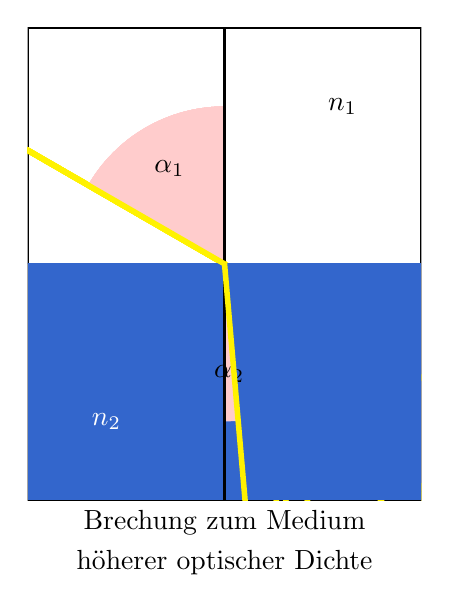
\begin{tikzpicture}[>=latex,thick]
\begin{scope}
	\clip (-2.5,-3) rectangle (2.5,3);
	\draw[color=black] (-2.5,-3) rectangle (2.5,3);
	\fill[color=darkblue] (-2.5,0) rectangle (2.5,-3);
	\uncover<4>{  \strahl{1.00}{20}    }
	\uncover<5>{  \strahl{1.34}{50}    }
	\uncover<6>{  \strahl{1.31}{45}    }
	\uncover<7>{  \strahl{1.57}{60}    }
	\uncover<8>{  \strahl{2.62}{70}    }
	\uncover<9>{  \strahl{3.45}{80}    }
	\uncover<10>{ \strahl{4.05}{90}    }
	\uncover<11->{ \strahl{10}{100}    }
	\uncover<2->{
		\node at (1.5,2) {$n_1$};
		\node[color=white] at (-1.5,-2) {$n_2$};
	}
\end{scope}
\uncover<14->{
	\node at (0,-3) [below] {Brechung zum Medium};
	\node at (0,-3.5) [below] {höherer optischer Dichte};
}
\end{tikzpicture}
\end{center}
\end{column}
\end{columns}
\end{frame}
\egroup
